% \newpage
\setcounter{section}{8}
\setcounter{subsection}{0}


\section{Scientific Essay: Thermalization and Localization}


\red{Lorem ipsum dolor sit amet, consectetur adipisicing elit, sed do eiusmod
tempor incididunt ut labore et dolore magna aliqua. Ut enim ad minim veniam,
quis nostrud exercitation ullamco laboris nisi ut aliquip ex ea commodo
consequat. Duis aute irure dolor in reprehenderit in voluptate velit esse
cillum dolore eu fugiat nulla pariatur. Excepteur sint occaecat cupidatat non
proident, sunt in culpa qui officia deserunt mollit anim id est laborum. 
EP-LP
Графики без ссылок получены мной
}




% ---------------------------
\subsection{Intro}


\textbf{Model}. We will study the effects of thermalization and localization using the Hubbard model 
\begin{equation}
	\hat{H} = 
	- J \sum_{\langle i,j\rangle} (\hat{a}_i\D \hat{a}_j + \hc) 
	+ V \sum_{\langle i,j\rangle} \hat{n}_i \hat{n}_j
	% + U 
	+ \Delta \sum_j \delta_j \hat{n}_j,
	\label{9:model}
\end{equation}
with $V$ -- nearest neighbor interaction, $\Delta$ -- noise level, $\delta_j \in [-1,1]$ evenly distributed (fig. \ref{fig:1Dmain}c). To obtain numerical results, the hard-bosons limit is used (unless explicitly stated otherwise)\footnote{
	The term $+ \tfrac{1}{2} U \sum_j \hat{n}_j (\hat{n}_j-1)$ was added to the Hamiltonian with $U \to \infty$. 
}.  This system is convenient in that we can look at various experimental implementations and all phases (EP and LP) of interest to us are implemented in it.





\begin{figure}[h]
    \centering
    \hspace{10 mm} 
    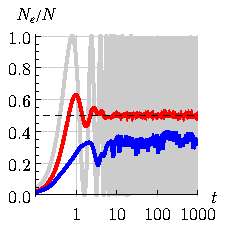
\includegraphics[align=c]{imgs/lo2.pdf}
    \hspace{1 mm} 
    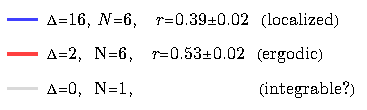
\includegraphics[align=c]{imgs/lo2l.pdf}
    \caption{
    An example of different behavior scenarios for some observable
    % $\hat{A} = \hat{N}_e / N$ при разных параметрах
    .
    }
    \label{fig:BASE}
\end{figure}



\textbf{Термализация}. Начнём с построения некоторой интуиции про то что можно было бы назвать термализацией для изолированной квантовой системы \cite{khlebnikov_thermalization_2014}. Пусть начальное состояние задаётся $\ket{\psi_0}$, тогда, in the basis of energy eigenstates $\ket{j}$, the evolution 
\begin{equation*}
	\ket{\psi(t)} = \sum_{j=1}^{\mathcal{N}} c_j e^{- i \varepsilon_j t} \ket{E_j}
\end{equation*}
with $c_j = \bk{E_j}{\psi_0}$, $\varepsilon_j = \bk{j}[\hat{H}]{j}$ and $\mathcal{N} = \dim H$. Для некоторой наблюдаемой $\hat{A}(t)$ the mean value could be expressed as 
\begin{equation}
	A(t) = \bk{\psi(t)}[\hat{A}]{\psi(t)} = \sum_{j,k} \bar{c}_k c_j e^{-i (\varepsilon_j - \varepsilon_k)} \bk{k}[\hat{A}]{j}
	=
	\sum_j |c_j|^2 \bk{j}[\hat{A}]{j} + \sum_{k \neq j} c_j \bar{c}_k e^{-i (\varepsilon_j - \varepsilon_k)} \bk{k}[\hat{A}]{j}.
	\label{eq:At}
\end{equation}
По прошествию некоторого времени термализации $\tth$ хотелось бы увидеть, что наблюдаемые выходят на термальные значения (независящие от начальных условий) с небольшими флуктуациями вокруг (fig. \ref{fig:BASE}, \red{red curve})
\begin{equation*}
	A(t \gg \tth) = A(E) + \text{small fluctuations},
	\hspace{10 mm} 
	E = \bk{\psi_0}[\hat{H}]{\psi_0}.
\end{equation*}
Для выхода на маленькие флуктуации вокруг среднего значения, как видим из \eqref{eq:At}, достаточно потребовать малости недиагональных элементов\footnote{
	Заметим, что диагональных слагаемых $\mathcal{N}$ и off-diagonal $\mathcal{N}^2- \mathcal{N}$. Если считать вклад каждого off-diagonal term случайным, то флуктуации может оценить, как $\sqrt{\mathcal{N}^2} |\bk{k}[\hat{A}]{j}|$, откуда и возникает требование малости.
}. 
% что и составляет первое условие Eigenstate Thermalization Hypothesis (ETH)
А чтобы $A(E)$ не зависело от начальных условий может рассмотреть случай, когда diagonal elements are smooth functions of energy
\begin{equation*}
	\bk{j}[\hat{A}]{j} = A(\varepsilon_j).
\end{equation*}
Действительно, тогда для начального состояния лежащего в $\Delta E $ such that the spread $\partial_E A(E) \Delta E$ is small, the final result is 
\begin{equation*}
	A(t \gg \tth) \approx \sum_j |c_j|^2 \bk{j}[\hat{A}]{j} \approx  A(E).
\end{equation*}
% \const + \text{fluctuations}
Так и приходим к формулировке Eigenstate Thermalization Hypothesis (ETH), put forward by Deutsch \cite{PhysRevA.43.2046} and Srednicki \cite{PhysRevE.50.888}: если off-diagonal terms $\bk{k}[\hat{A}]{j}$ are small in compared to diagonal and diagonal terms are smooth functions of energty, то наблюдаемая как будто бы термализуется.  Стоит сделать некоторую оговорку, что для изолированной системы чистое состояния остаётся чистым $\tr \rho^2 = 1$, в то время как для термального состояния $\tr \rho^2 < 1$, поэтому и говорим о термализации наблюдаемых\footnote{
	Возникает надежда, что если мы будем разобьём систему на две подсистемы $\Omega_1 \cup \Omega_2$, то $\rho_1 = \tr_{\Omega_2} \rho$ уже действительно может оказаться термальной, а $\Omega_2$ выступает в некотором смысле термостатом для $\Omega_1$. Данное предположение не получит развития в рамках этого эссе, однако автор надеется вернуться к этому вопросу позднее.
}. Опять же, судя по условиям, как будто бы возможны системы и наблюдаемые $A_1,\, A_2$ такие что $A_1$ термализуется, а $A_2$ нет. 

Основной вывод этого раздела: иногда так бывает, что в некоторой системе и для некоторой наблюдаемой $\hat{A}$ её значение $A(t \gg \tth)$ выходит на константу с небольшими флуктуациями вокруг, скорее всего этому будут соответсвовать указанные ETH условия.


% , что для short-range наблюдаемой, для вычисления которой можно разбить систему на подситемы и найти $A$ в них, 

\textbf{Локализация}. Принципиально противоположным термализации будет локализация. Так бывает, что система сохраняет информацию о начальных условиях даже при $t \to \infty$ (fig. \ref{fig:BASE}, \blue{blue curve}) и $A = A(\psi_0)$.  Например мы можем разделить систему на две равные подсистемы $\Omega_1,\, \Omega_2$, заселить только $\Omega_1$ и следить за контрастностью
\begin{equation*}
	\mathcal{I} = \frac{N_{\Omega_1}-N_{\Omega_2}}{N_{\Omega_1}+N_{\Omega_2}}.
\end{equation*}
Так в \cite{schreiber_observation_2015} в 1D в качестве $\Omega_1$ выбрали чётные узлы решётки (fig. \ref{fig:loc1}), а в \cite{Choi_2016} в 2D за $\Omega_1$ взяли левую часть системы (fig. \ref{fig:loc2D1}). Как раз для $\mathcal{I}(t)$ уже видно заявленное термальное поведение, когда $\mathcal{I}(t \gg \tth) \approx 0$, но в какой-то момент случается переход к локализации и $\mathcal{I} (t \gg \tth) \approx \const > 0$. Такое поведение характерно при добавление в систему frozen noise $\Delta > 0$, первые данный эффект был описан by Anderson \cite{PhysRev.109.1492}.

Для одночастичной задачи было бы логичным предположить, что такое поведение возникает из-за локализации собственных функций. Действительно, в fig. \ref{fig:loc1} представлены собственные состояния гамильтониана при разных уровнях шума.  

% Здесь хотелось бы добавить немного конкретики, в этом эссе будет рассматриваться Hubbard model (которая иногда сводится к Heisenberg model, см. приложение):



\begin{figure}[h]
    \centering
    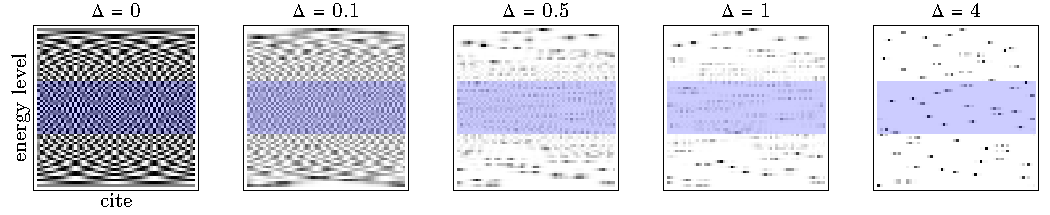
\includegraphics{imgs/evecs.pdf}
    \caption{Eigenvectors for $L=60$ and $N=1$}
    \label{fig:loc1}
\end{figure}


% ---------------------------




% \newpage
% ---------------------------
\subsection{MBL experiment in 2D}

Let's consider the experimental implementation of the \eqref{9:model} system in \cite{Choi_2016} with approximately unity filled Mott insulator of bosonic ${}^{87}$Rb atoms in a single plane of a cubic optical lattic. 


To do this, by combining laser beams, we will obtain a certain interference pattern, the antinodes of which, at red detuning, will act as minima of the potential for atoms due to their polarizability (an alternative would be a lattice of optical tweeters). Between these potential minima, atoms will tunnel with a characteristic energy $J$ (as in fig. \ref{fig:1Dmain}c), which we will use as an energy scale. We can adjust the interaction $U$ between atoms using Feischbach resonances, by turning it up to the value $U=24J$ we get a system close to hard-bosons. We will apply a global harmonic potential on top of the grating, also by focusing the laser. Let's fill the trap with sufficiently cold atoms, using a microwave knife, leave only the left half filled and wait a little (fig. \ref{fig:loc2D1}). Noises $\Delta$ are added to the system using DMD (alternatively, SLM, AOD or quasi-random potential are used as in \cite{schreiber_observation_2015}, more details in \cite{abanin_many-body_2019}), the result is averaged over 50 implementations of $\delta_j$.

\begin{figure}[h]
    \centering
    \addletter{80}{a}
    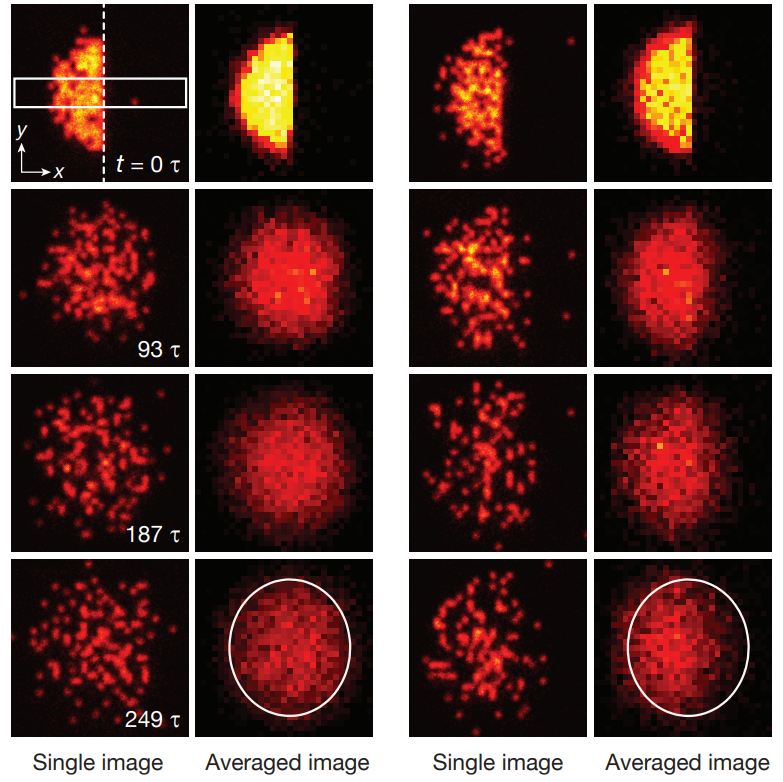
\includegraphics[align=c, width=0.33\textwidth]{imgs/MBL_2D_exp_1.png}
    \hspace{10 mm} 
    \addletter{80}{b}
    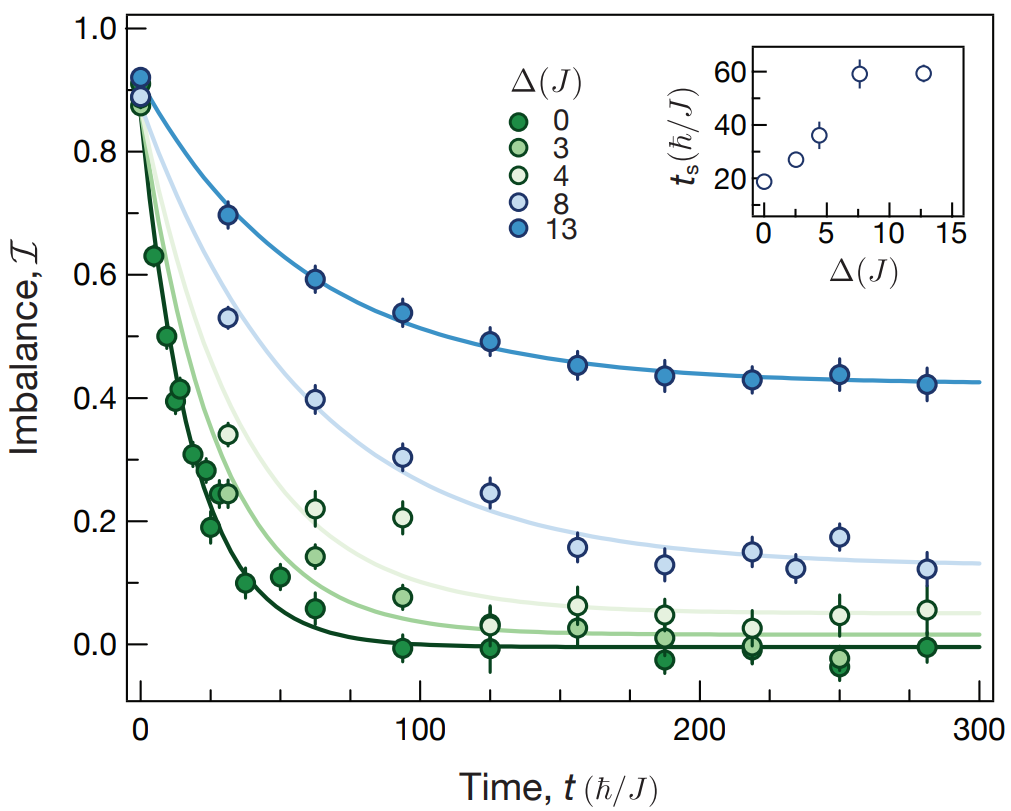
\includegraphics[align=c, width=0.4\textwidth]{imgs/MBL_2D_exp_2.png}
    % 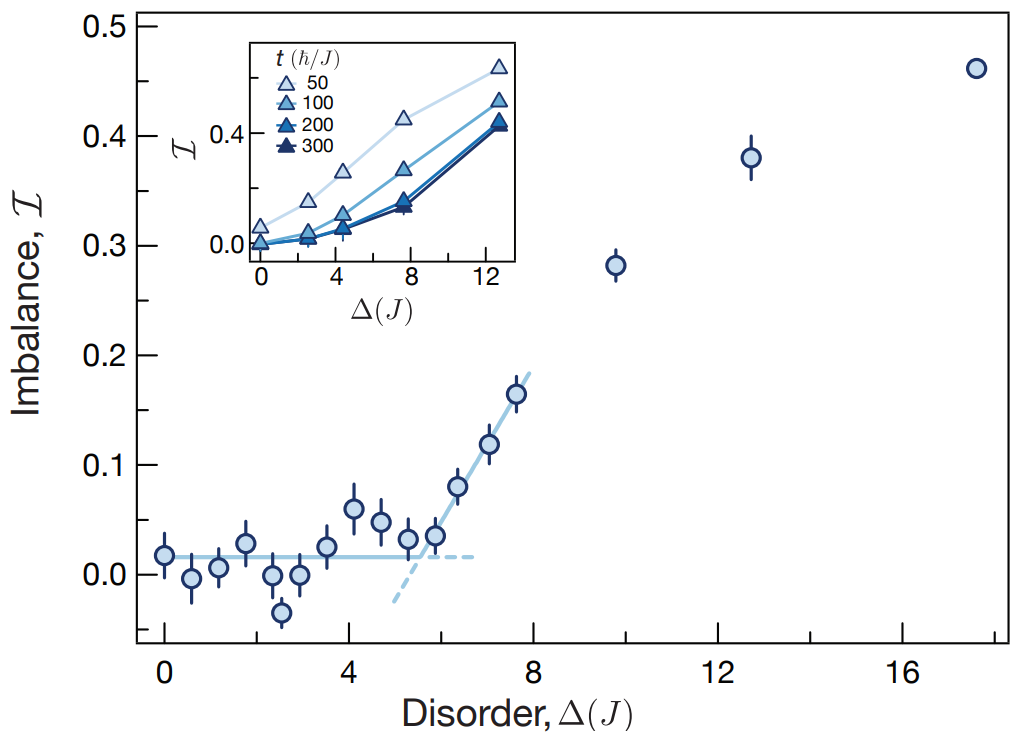
\includegraphics[align=c, width=0.4\textwidth]{imgs/MBL_2D_exp_3.png}
    \caption{
        \cite{Choi_2016}
        a) Raw fluorescence images (red to yellow corresponds to increasing detected light level) showing the evolution of the initial density step without disorder. The left column shows the evolution with $\Delta=0$ and the right column $\Delta = 13 J$.
        b) Relaxation dynamics of a density domain wall.
    }
    \label{fig:loc2D1}
\end{figure}


It can be seen that in the absence of noise the system reaches a thermal state - thermalization ($\mathcal{I} \to 0$). With sufficiently strong noise, localization occurs: $\mathcal{I}(t \to \infty) = \mathcal{I}_\infty > 0$. Assuming the output to $\mathcal{I}_\infty$ to be exponential, we can notice how what is required to reach a steady state increases as the noise level increases.


It can also be seen that $\mathcal{I}_\infty > 0$ appears with $\sub{\Delta}{c} \approx 5.5(4) J$. The article emphasizes that $\sub{\Delta}{c}$ will increase as initial filling decreases. The clear difference in critical disorder strengths highlights the strong influence of interactions on the localization.



% ---------------------------




% ---------------------------
\subsection{MBL experiment in 1D}

Для демонстрации перехода EP-LP можем рассмотрим также эксперимент по реализации одномерной системы \cite{schreiber_observation_2015}. Теперь рассматривается движение в quasi-random optical lattice созданной двумя решетками с несоизмерным шагом, но в целом всё также описывающейся гамильтонианом \eqref{9:model}.



\begin{figure}
    \centering
    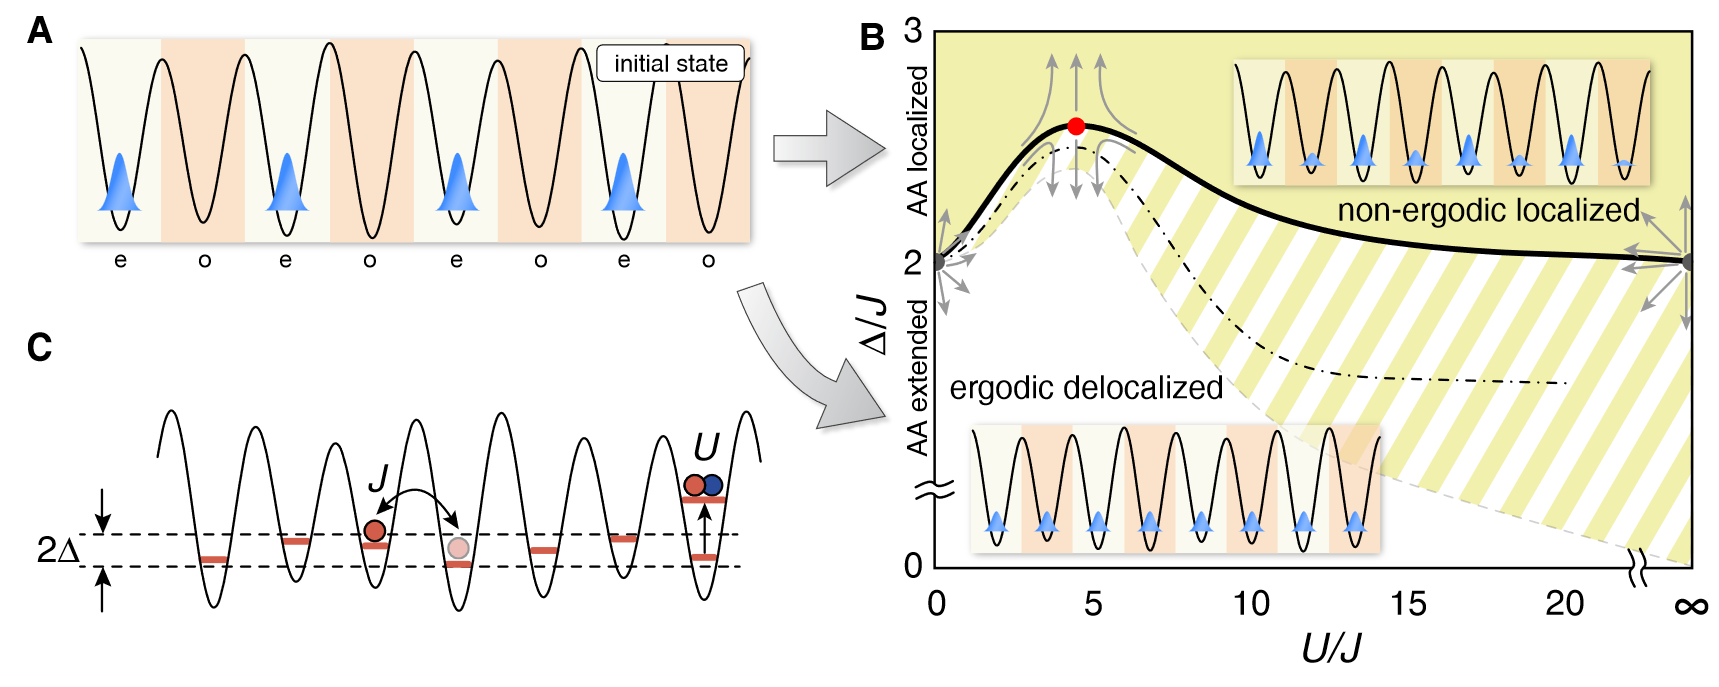
\includegraphics[width=0.7\textwidth]{imgs/1d_phases.png}
    \caption{\cite{schreiber_observation_2015} a) Initial state of the system consisting of a charge density wave, where all atoms occupy even sites only. For an interacting many-body system, the evolution of this state over time depends on whether the system is ergodic or not. b) Schematic phase diagram for the system: in the ergodic, delocalized phase (white) the initial state quickly decays, while it persists for long times in the non-ergodic, localized phase (yellow). c) Schematic showing a visual representation of the three terms in the Hamiltonian. }
    \label{fig:1Dmain}
\end{figure}




Теперь в качестве $\Omega_1$ выбраны нечётные узлы и также исследуется на сколько быстро исчезнет и до какой степени контрастность $\mathcal{I}$ заселенности чётных и нечётных узлов (fig. \ref{fig:loc1D1}). Видно, что за $t \approx 15 \tau$ наблюдаемая $\mathcal{I}$ также выходит на стационарное значение (fig. \ref{fig:loc1D1}a), где по результатм усреднения в желтой области строится зависимость $\mathcal{I}(\Delta)$ (fig. \ref{fig:loc1D1}b).

\begin{figure}
    \centering
    \addletter{45}{a}
    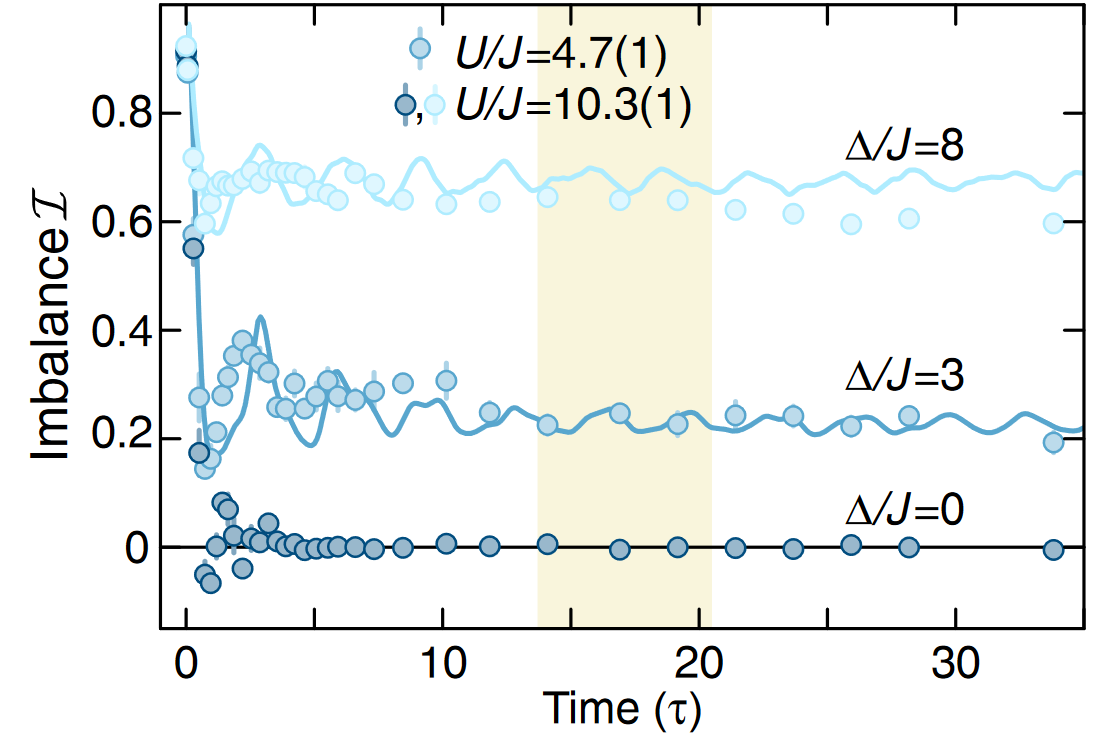
\includegraphics[align=c, width=0.35\textwidth]{imgs/MBL_exp_1.png}
    \hspace{10 mm} 
    \addletter{45}{b}
    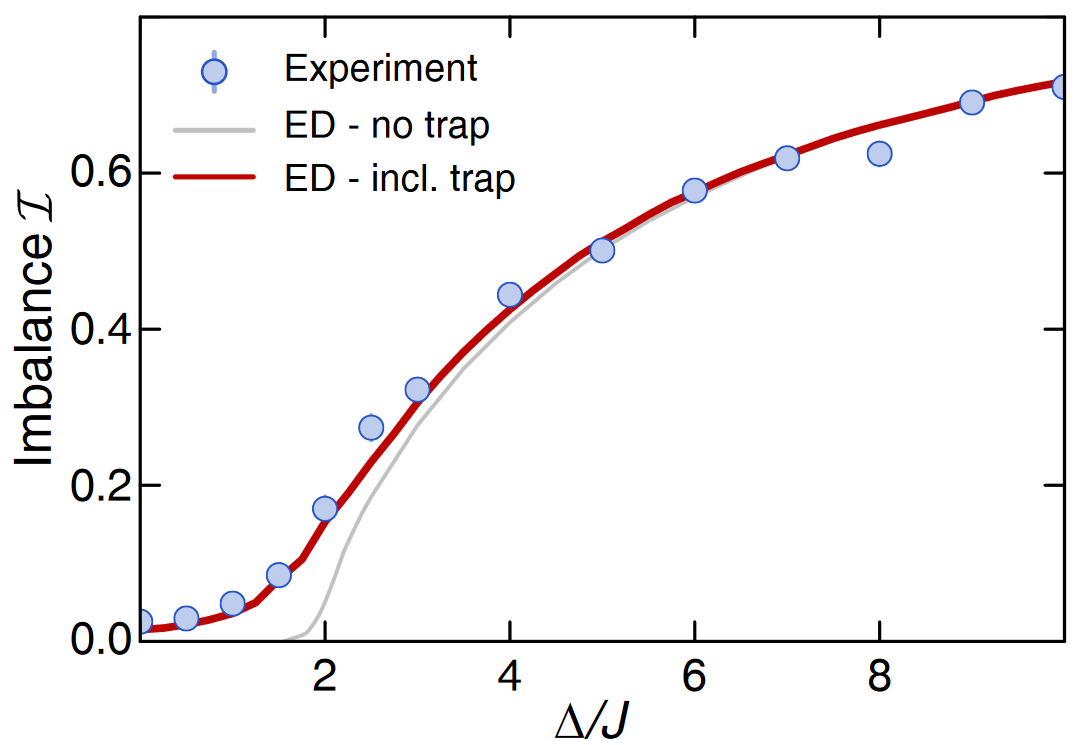
\includegraphics[align=c, width=0.35\textwidth]{imgs/MBL_exp_2.png}
    \caption{
    \cite{schreiber_observation_2015} 
    a) Time evolution of an initial charge-density wave
    . 
    b) Stationary values of the imbalance $\mathcal{I}$ as a function of disorder $\Delta$ for non-interacting atoms 
    .
    }
    \label{fig:loc1D1}
\end{figure} 





% \red{Основной вывод от этой картинки и этой статьи: есть локализация и термолизация. Взаимодействие влияет, но не столь принципиально.}}
% ---------------------------




% ---------------------------
\subsection{Numerical model in 2D}

\begin{figure}[h]
    \centering
    \addletter{115}{a}
    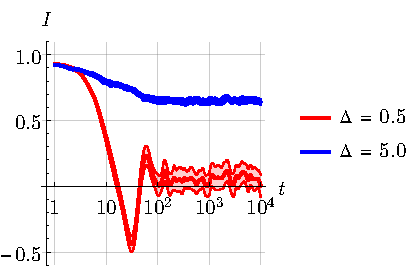
\includegraphics{imgs/2Dth_loc.pdf}
    % \hspace{5 mm} 
    \addletter{115}{b}
    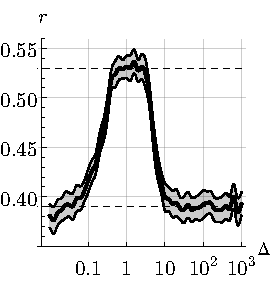
\includegraphics{imgs/2Drdel.pdf}
    % \hspace{5 mm} 
    \addletter{115}{c}
    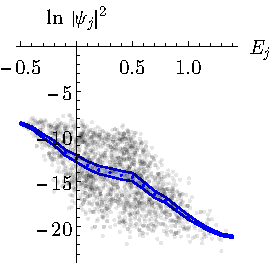
\includegraphics{imgs/2Dtherm_1.pdf}
    \caption{a) ... b) ... c) ... }
    \label{fig:2Dtherm}
\end{figure}


\begin{figure}[h]
    \centering
    \addletter{80}{a}
    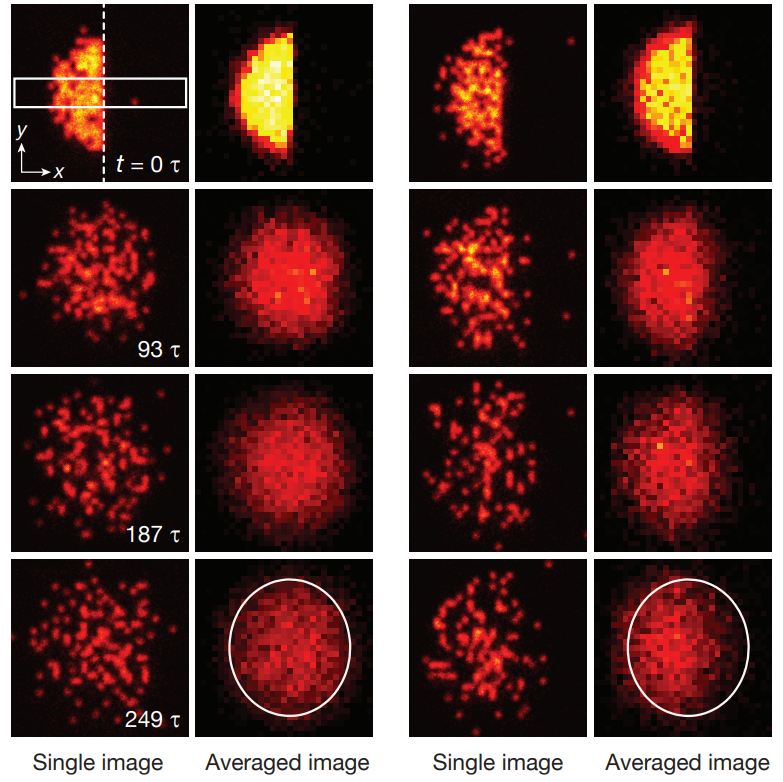
\includegraphics[align=c, width=0.33\textwidth]{imgs/MBL_2D_exp_1.png}
    \hspace{10 mm} 
    \addletter{80}{b}
    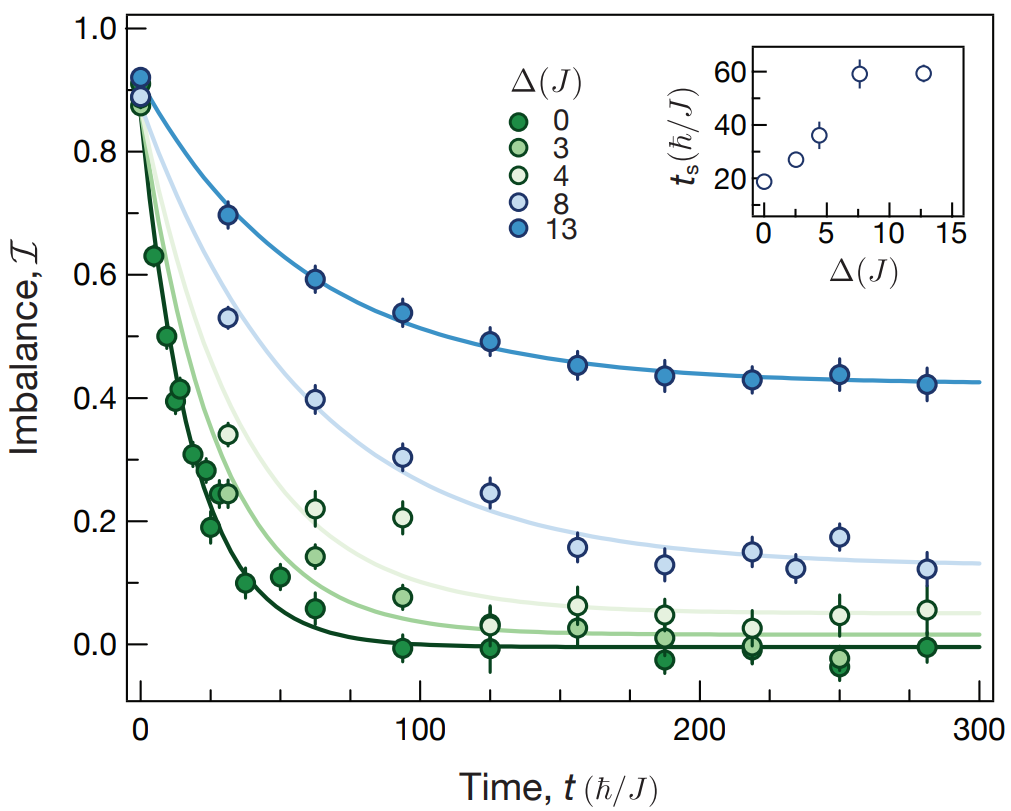
\includegraphics[align=c, width=0.4\textwidth]{imgs/MBL_2D_exp_2.png}
    % 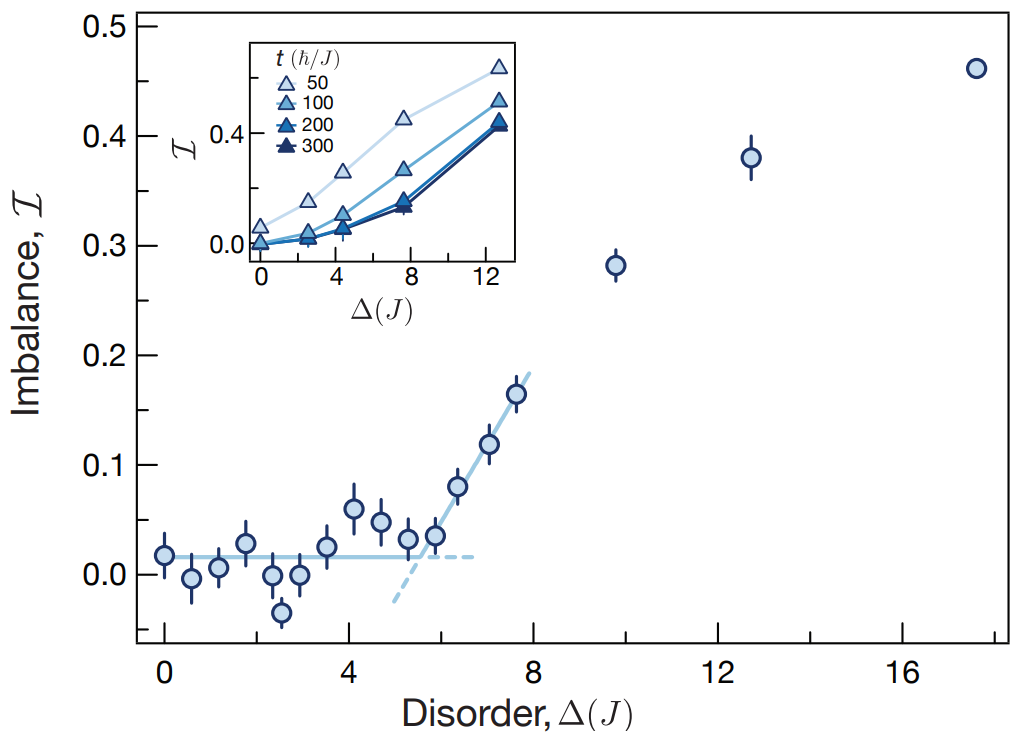
\includegraphics[align=c, width=0.4\textwidth]{imgs/MBL_2D_exp_3.png}
    \caption{
        a) Raw fluorescence images (red to yellow corresponds to increasing detected light level) showing the evolution of the initial density step without disorder \cite{Choi_2016} . 
        b) Relaxation dynamics of a density domain wall \cite{Choi_2016} .
    }
    \label{fig:loc2D1}
\end{figure}


% experimental implementation of the model
% ---------------------------




% \newpage
% ---------------------------
\subsection{Random Matrices}

Давайте рассмотрим следующую процедуру: для некоторой матрицы $M$ найдём все собственные числа $\lambda_j$, упорядоченные по возрастанию, и определим $r$-параметр \cite{wei_characterization_2020} 
\begin{equation*}
    r \overset{\mathrm{def}}{=}  \left\langle \frac{\min(\delta_j, \delta_j+1)}{\max(\delta_j, \delta_{j+1})} \right\rangle_j,
    \hspace{10 mm} 
    \delta_j = \lambda_{j+1}-\lambda_j.
\end{equation*}
Сразу можем отметить несколько таких свойств, что он не чувствителен к преобразованиям вида $M \to \alpha_1 M + \alpha_2 \1$, более того как позже заметим он много к чему не чувствителен. 


\begin{figure}[tb]
    \centering
    \addletter{107}{a}
    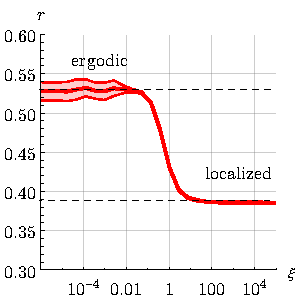
\includegraphics[width=0.225\textwidth]{imgs/erg_reg_add1.pdf}
    \hspace{10 mm} 
    \addletter{107}{b}
    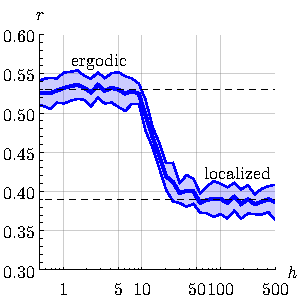
\includegraphics[width=0.225\textwidth]{imgs/erg_reg_add2.pdf}
    \caption{a) Phase transition EP-LP with random matrix. b)  Phase transition EP-LP with 1D hard-bosons \eqref{9:model}, $h \equiv \Delta$}
    \label{fig:rxi}
\end{figure}


Теперь посмотрим подробнее на систему \eqref{9:model} и фазовый переход, который случается при повышении $\Delta$. В координатном представлении шумы являются просто случайной диагональной добавкой к гамильтониану\footnote{
    Тут нужно быть аккуратным, потому что как мы увидим позднее, небольшим изменения диагонали через $V \neq 0$ приводят к принципиально другому поведению системы \cite{bardarson_unbounded_2012}. 
}. Таким образом при $\Delta \gg J$ (по крайней мере в одночастичном случае) гамильтониан практически диагонализуется (fig. \ref{fig:loc1}). С другой стороны есть недиагональная часть, за которую отвечает $J$. В статье \cite{wei_characterization_2020} предлагается моделировать этот фазовый переход с помощью двух случайных матриц: случайной эрмитововой $M_1$ (GOE) и случайной диагональной $M_2$, таким образом $M = (1-k) M_1 + k M_2$. The limiting values $k=0$ and $k=1$ characterize chaotic and nonchaotic regimes (термализующийся и локализующийся). Чтобы переход не зависел от параметров $M_{1,2}$ можем scale $k$ as
\begin{equation*}
    \xi = \frac{1}{D} \frac{k \sigma_2}{(1-k)\sigma_1},
\end{equation*}
where $\sigma_{1,2}$ are the standard deviation of elements in $M_{1,2}$ respectively and $D$ is the size of the matrix. 

Найдём, как зависит $r(\xi)$ для матриц при $D=200$, $\sigma_1=\sigma_2=1$ (для других значений зависимость такая же), усредняя результат по 100 реализациям (fig. \ref{fig:rxi}a). Для сравнения приведена зависимость $r(\xi)$ для 1D системы \eqref{9:model} hard-bosons по уровню шума $h$ (то же самое, что и $\Delta$) на решётке в $L=14$ узлов с половинным заполнением\footnote{
    Если бы мы говорили про Heisenberg model, то это соотвествовало полному спину равному нулю. 
} (7 частицами).  В соответсвии с \cite{wei_characterization_2020, pal_many-body_2010} значение $r \approx 0.53$ является маркером эргодической фазы (характерное значение для GOE), а $r \approx 0.39$ является маркером локализованной фазы (так называемая Poisson statistics):
\begin{equation*}
\boxed{
    r \approx 0.53 \text{ -- ergodic}
}
\hspace{10 mm} 
\boxed{
    r \approx 0.39 \text{ -- localized}
}
\end{equation*}
Замечу, что используется именно слово маркер, так как эти условия не являются необходимыми и не являются достаточными. 

\begin{figure}
    \centering
    \addletter{50}{a}
    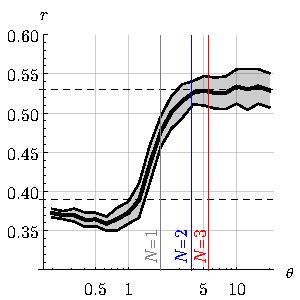
\includegraphics[align=c, width=0.225\textwidth]{imgs/ergodic_reg.pdf}
    \hspace{10 mm} 
    \addletter{50}{b}
    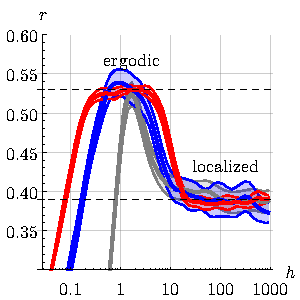
\includegraphics[align=c, width=0.225\textwidth]{imgs/transition.pdf}
    \hspace{5 mm} 
    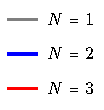
\includegraphics[align=c, width=0.075\textwidth]{imgs/transition_leg.pdf}
    \caption{
        a) The influence of matrix rarefaction $\theta$ on phase formation. 
        b) Phase transition with 1D hard-bosons 
    % N=200
    % $\xi=0.01$, $L=20$
    }
    \label{fig:rtheta}
\end{figure}

 

% \cite{pal_many-body_2010} -- The many-body localization phase transition


Аналогичная зависимость получится, если в качестве $M_1$ будем рассматривать матрицу связности случайного графа (эрмитова матрица со случайными элементами $0,1$). 
Считая, что в среднем на строчку приходится $\theta$ ненулевых элементов, можем задаться вопросом о влиянии $\theta$ на формировании эргодической фазы (fig. \ref{fig:rtheta}a). При слишком маленьких $\theta$ высока вероятность Hilbert Space Fragmentation \cite{Moudgalya_2022}, что очевидно не может давать термализацию системы. Тем более система не термализуется, когда является интегрируемой \cite{rigol_thermalization_2008}.

Такое внимание к $\theta$ и фрагментации уделил, так как это в каком-то смысле помогает понять, почему для небольшого числа частиц в системе эргодическая фаза (судя по $r$) практически не наступает (fig. \ref{fig:rtheta}). Действительно, при меньшем числе частиц ($N=1,2,3$) и том же размере решётки $L=14$ гамильтониан более разряженный (fig. \ref{fig:rtheta}a), происходит Hilbert Space Fragmentation (то есть гамильтониан можно представить в блочно диагональном виде) и, соответсвенно, не происходит термализации. 


Основной вывод этого раздела: $r$-параметр носит достаточно универсальный характер, может использоваться как маркер эргодичной фазы и локализованной фазы. Фазовый переход EP-LP может моделироваться случайными матрицами (GOE, random diagonal, random graph adjacency matrix).
% ---------------------------




% ---------------------------
\subsection{Numerical model in 1D}



\begin{figure}[h]
    \centering
    \addletter{45}{a}
    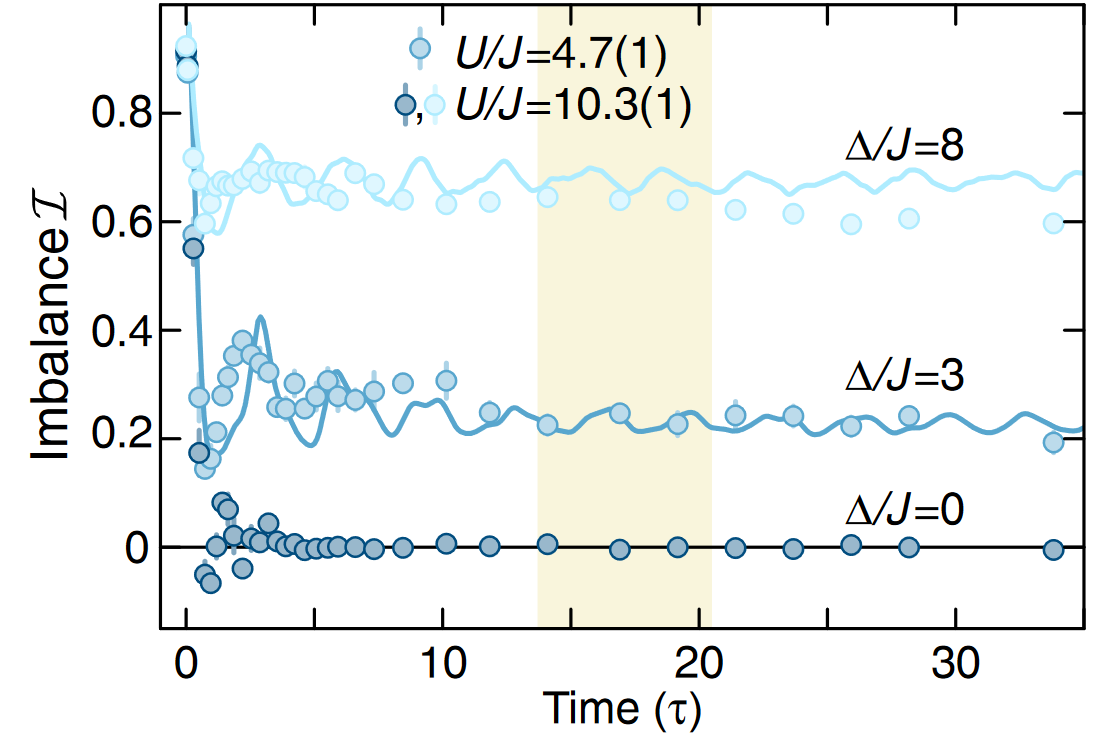
\includegraphics[align=c, width=0.35\textwidth]{imgs/MBL_exp_1.png}
    \hspace{10 mm} 
    \addletter{45}{b}
    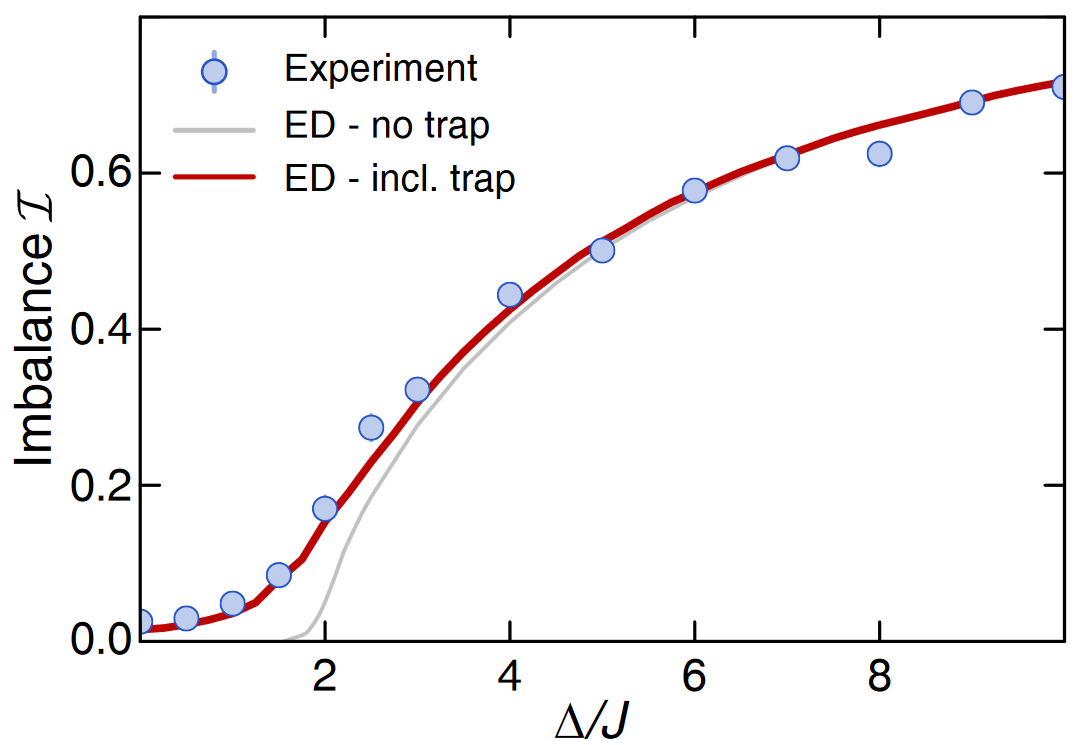
\includegraphics[align=c, width=0.35\textwidth]{imgs/MBL_exp_2.png}
    \caption{
    a) Time evolution of an initial charge-density wave
    \cite{schreiber_observation_2015} 
    . 
    b) Stationary values of the imbalance $\mathcal{I}$ as a function of disorder $\Delta$ for non-interacting atoms 
    \cite{schreiber_observation_2015} 
    .
    }
    \label{fig:loc1D1}
\end{figure}

% \red{Основной вывод от этой картинки и этой статьи: есть локализация и термолизация. Взаимодействие влияет, но не столь принципиально.}}
% ---------------------------



% \newpage
% ---------------------------
\subsection{Entropy growth}


\begin{figure}[h]
    \centering
    \addletter{50}{a} \hspace{2 mm} 
    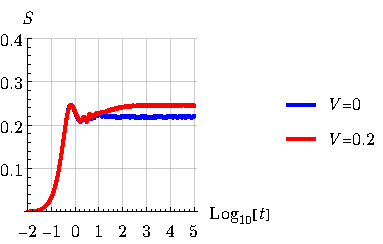
\includegraphics[align=c]{imgs/S_FV1.pdf}
    \hspace{10 mm} 
    \addletter{50}{b} \hspace{2 mm} 
    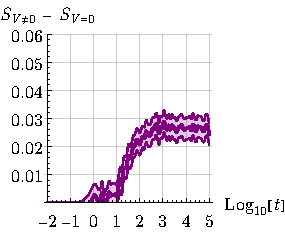
\includegraphics[align=c]{imgs/S_FV2.pdf}
    \caption{a) Entanglement growth. b) The same data but with subtracted values.}
    %\label{fig:}
\end{figure}




\begin{figure}[h]
    \centering
    \addletter{150}{a} 
    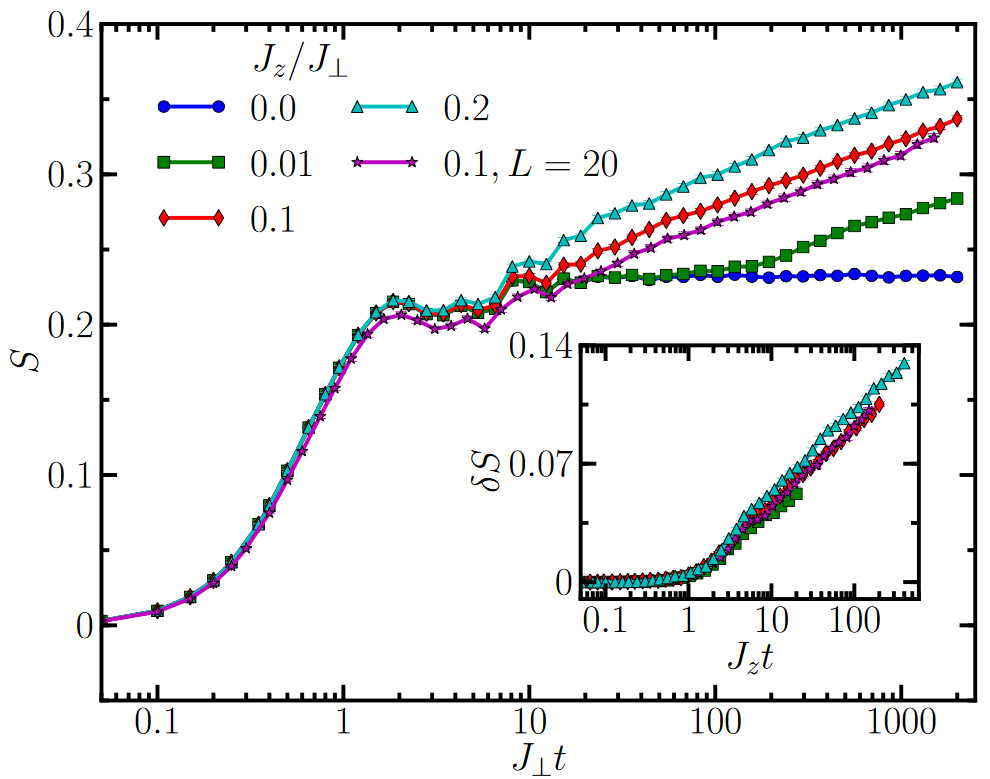
\includegraphics[width=0.4\textwidth]{imgs/S_FV_12a.png}
    \hspace{10 mm} 
    \addletter{150}{b} 
    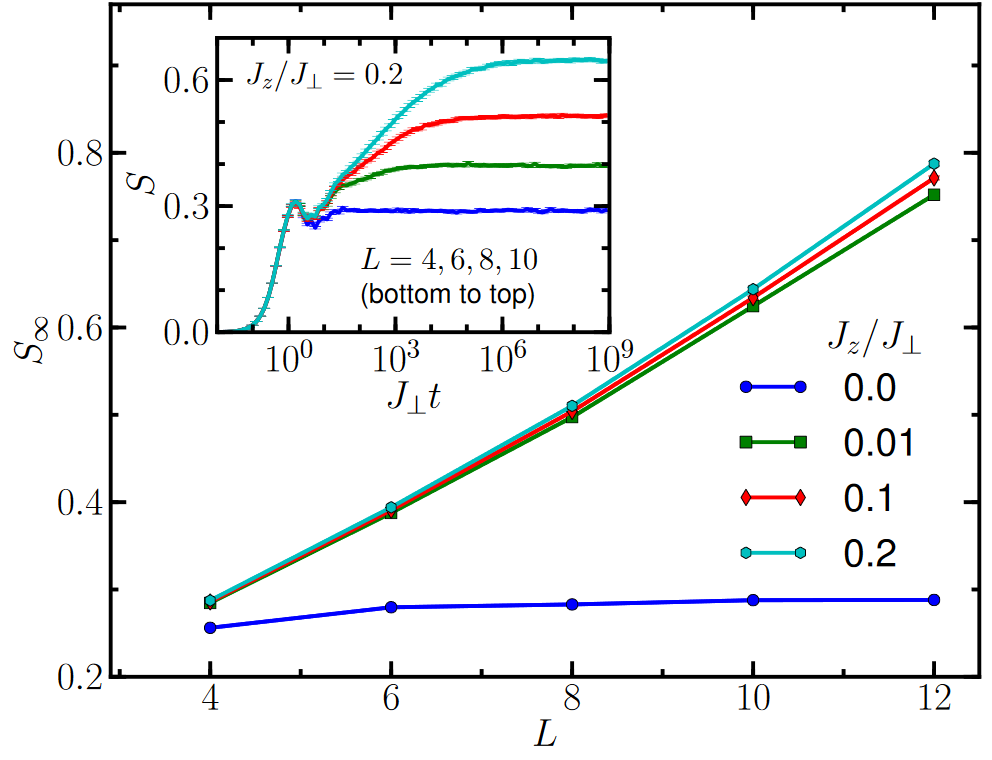
\includegraphics[width=0.4\textwidth]{imgs/S_FV_12b.png}
    \caption{
        a) Entanglement growth \cite{bardarson_unbounded_2012}.
        b) Saturation values of the entanglement entropy as a function of $L$ \cite{bardarson_unbounded_2012}.
    }
    %\label{fig:}
\end{figure}

% ---------------------------




% \newpage
% ---------------------------
\subsection{Conclusion}

Experimental implementations and numerical simulations of EP and LP in the Hubbard model (or in 1D Heisenberg model) in 1D and 2D for the non-interacting case (EP-LP:AL) and the interacting case (EP-LP:MBL) are considered.
For a many-particle problem, the Hamiltonian is less sparse;
Hilbert Space Fragmentation, but thermalization usually occurs. A shift in the critical noise level required for transition to LP was observed due to the presence of interactions between particles. Also, fundamentally different behavior was observed in MBL compared to AL in terms of the growth of entanglement and entropy of subsystems.
% ---------------------------




% ---------------------------
% \subsection{Experimental implementations}

% \input{parts/hw9_}
% ---------------------------








% ---------------------------

\newpage
\subsection{Supplementary Material}









\begin{figure}[h]
    \centering
    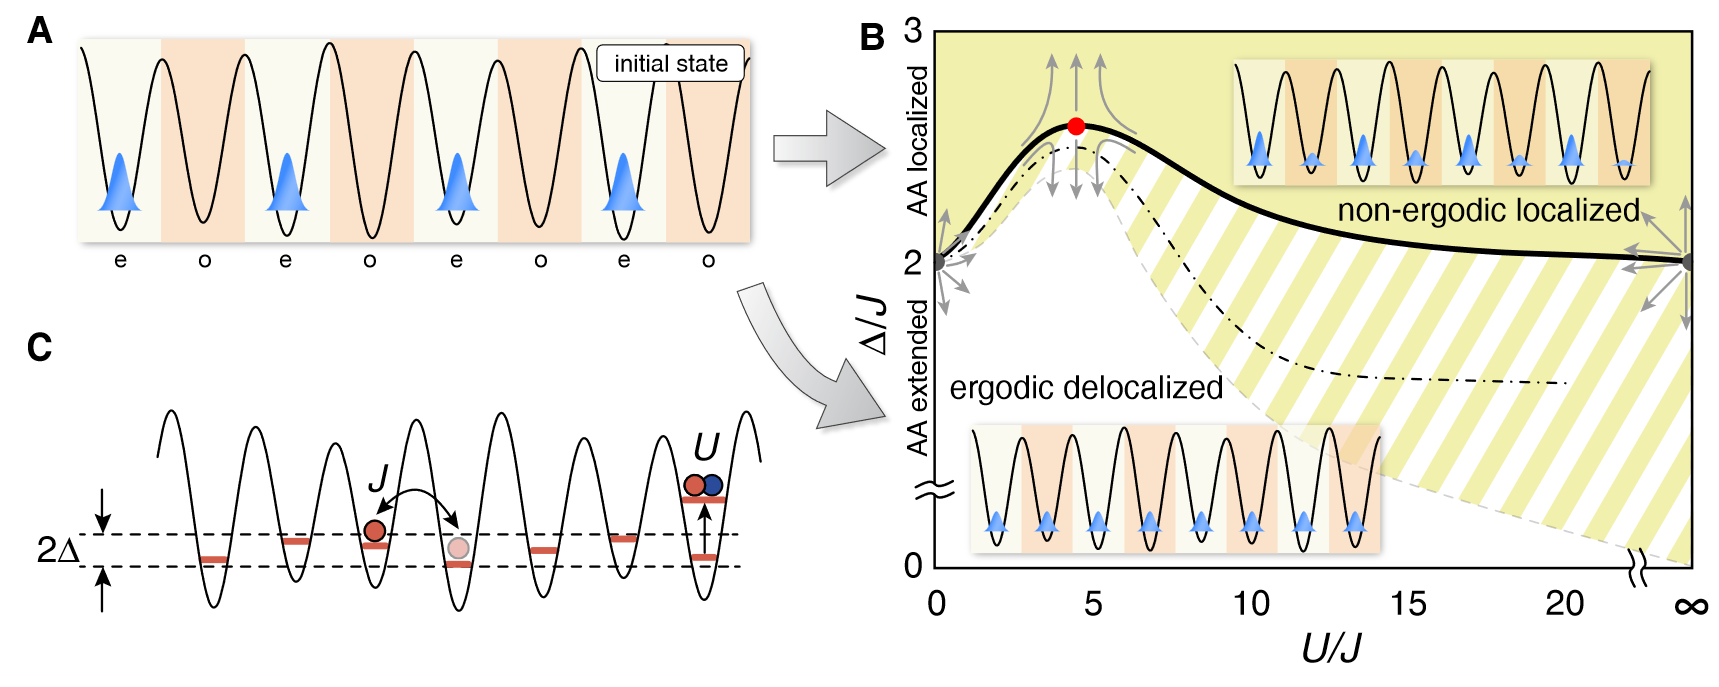
\includegraphics[width=0.7\textwidth]{imgs/1d_phases.png}
    \caption{\cite{schreiber_observation_2015} 1D system \eqref{9:model}. a) Initial state of the system consisting of a charge density wave, where all atoms occupy even sites only. For an interacting many-body system, the evolution of this state over time depends on whether the system is ergodic or not. b) Schematic phase diagram for the system: in the ergodic, delocalized phase (white) the initial state quickly decays, while it persists for long times in the non-ergodic, localized phase (yellow). c) Schematic showing a visual representation of the three terms in the Hamiltonian \eqref{9:model}. }
    \label{fig:1Dmain}
\end{figure}






\begin{figure}[h]
    \centering
    \addletter{75}{a} 
    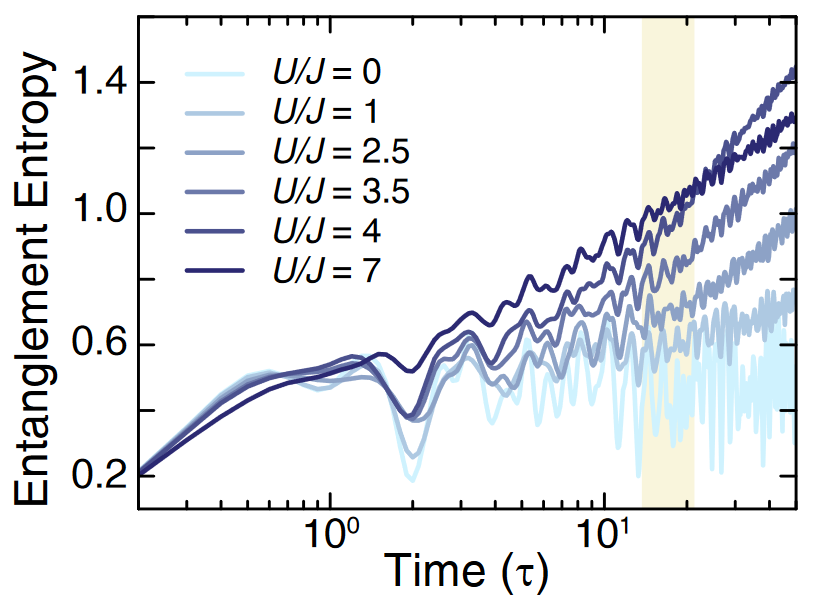
\includegraphics[align=c, width=0.35\textwidth]{imgs/1d_add1.png}
    \hspace{10 mm} 
    \addletter{75}{b} 
    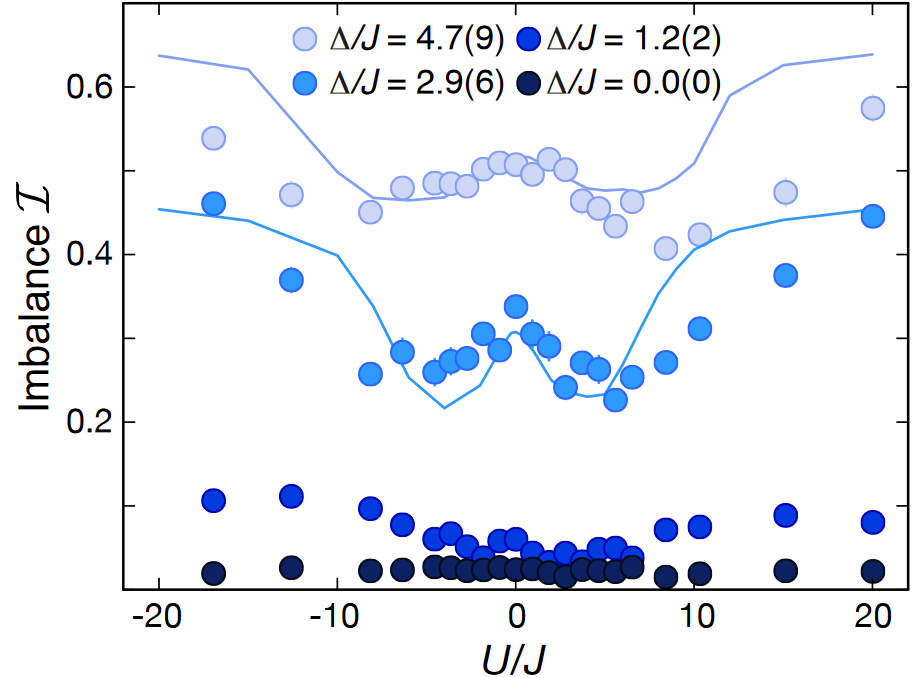
\includegraphics[align=c, width=0.4\textwidth]{imgs/1d_add2.png}
    \caption{
    \cite{schreiber_observation_2015}
        a) DMRG results of the entanglement entropy growth for various interaction strengths and $\Delta = 5 J$. For long times, logarithmic growth characteristic of interacting MBL states is visible.
        b) Cuts along four different disorder strengths. The effect of interactions on the localization gives rise to a characteristic W-shape. Solid lines are the results of DMRG simulations for a single homogeneous tube. 
    }
    \label{fig:1daddb}
\end{figure}







\newpage
% План эссе

% \begin{itemize}
% 	\item Введение 



% 	\item 
% \end{itemize}

% \newpage


% \cite{pal_many-body_2010} -- The many-body localization phase transition

% \cite{schreiber_observation_2015} -- Observation of many-body localization of interacting fermions in a quasi-random optical lattice









% \addcontentsline{toc}{section}{Список литературы}
\bibliography{MBL}

% \newpage



% % ---------------------------

% В этом эссе рассмотрим добавление frozen noise в различные системы.
 % при разной температуре и разной размерности. 
В частности убедимся в возникновение двух противоположных эффектов: \textit{термолизации} (иногда возникающей при небольшом уровне шума) и \textit{локализации} (при <<достаточном>> уровне шума). 

\red{Отлельный сюжет -- рост запутанности подсистем. Построить мостик со статьей, поговорить про $\tr \rho^2$ для подсистемы. Посмотреть на термальность матрицы плотности подсистемы.}

% Для полноты изложения и формирования первичной интуиции начнём с одночастичной задачи и андерсоновской локализации. 

Наличие шума приводит к неинтегрируемости системы, и иногда в этой изолированной квантовой системе в некотором смысле возникает термолизация. 
Что значит интерируемая квантовая система? Что такое \textit{термолизация}? Что такое \textit{ETH}?
Что такое \textit{локализация}? 
И к любому эффекту возникает вопрос какими метриками мы можем его охарактеризовать? Являются ли они достаточными и необходимыми? В чём принципиальное отличие MBL от Андерсоновской локализации?
\red{Хочется определить основные понятия, продемонстривовать как это всё работает. Потом в дополнение можно прокомментировать отдельные графики из статей} 


	
Рассмотрим one-dimensional Fermi-Hubbard model with 
\begin{equation*}
	\hat{H} = 
	- J \sum_{\langle i,j\rangle} (\hat{a}_i\D \hat{a}_j + \hc) 
	+ \Delta \sum_j \varepsilon_j \hat{n}_j
	+ V \sum_{\langle i,j\rangle} \hat{n}_i \hat{n}_j,
\end{equation*}
with равномерно-случайными $\varepsilon_j \in [-1,1]$. Эта система удобна тем, что можем посмотреть на различные экспериментальные реализации и в ней реализуются все интересные нам режимы. Я не буду здесь лезть в интегрируемые квантовые системы, и так хватает открытых вопросов. 



% Our main observable is the imbalance $I$ between the respective atom numbers on even ($N_e$) and odd ($N_o$) sites
% \begin{equation*}
% 	I = \frac{N_e - N_o}{}
% \end{equation*}

% J=1,V=0.5




\begin{figure}[h]
    \centering
    % 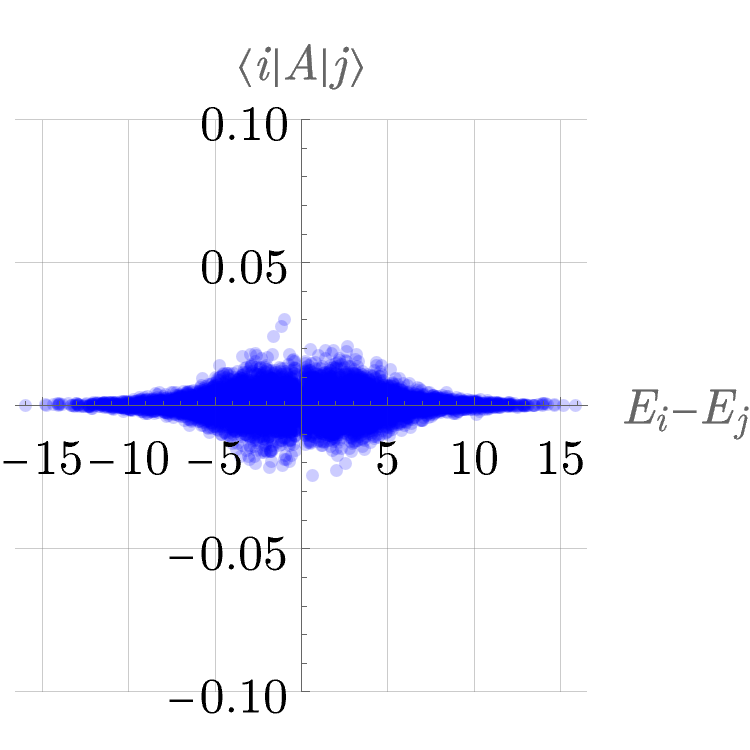
\includegraphics[align=c, width=0.25\textwidth]{imgs/lo1.png}
    \hspace{10 mm} 
    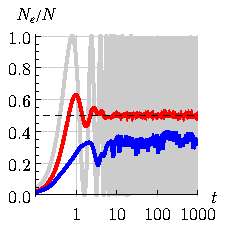
\includegraphics[align=c]{imgs/lo2.pdf}
    \hspace{1 mm} 
    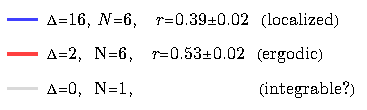
\includegraphics[align=c]{imgs/lo2l.pdf}
    \caption{labore et dolore magna aliquat enim ad minim veniam with $L=12$}
    %\label{fig:}
\end{figure}

Lorem ipsum dolor sit amet, consectetur adipisicing elit, sed do eiusmod
tempor incididunt ut labore et dolore magna aliqua. Ut enim ad minim veniam,
quis nostrud exercitation ullamco laboris nisi ut aliquip ex ea commodo
consequat. Duis aute irure dolor in reprehenderit in voluptate velit esse
cillum dolore eu fugiat nulla pariatur. Excepteur sint occaecat cupidatat non
proident, sunt in culpa qui officia deserunt mollit anim id est laborum.



\begin{figure}[h]
    \centering
    \addletter{45}{a}
    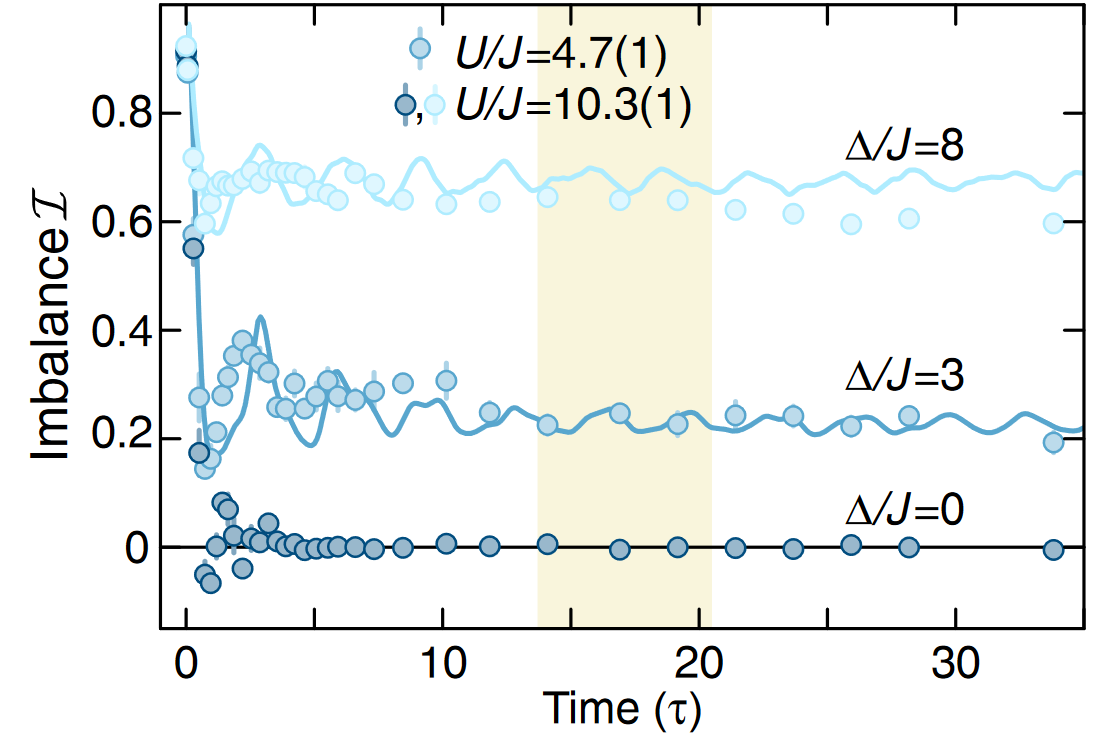
\includegraphics[align=c, width=0.35\textwidth]{imgs/MBL_exp_1.png}
    \hspace{10 mm} 
    \addletter{45}{b}
    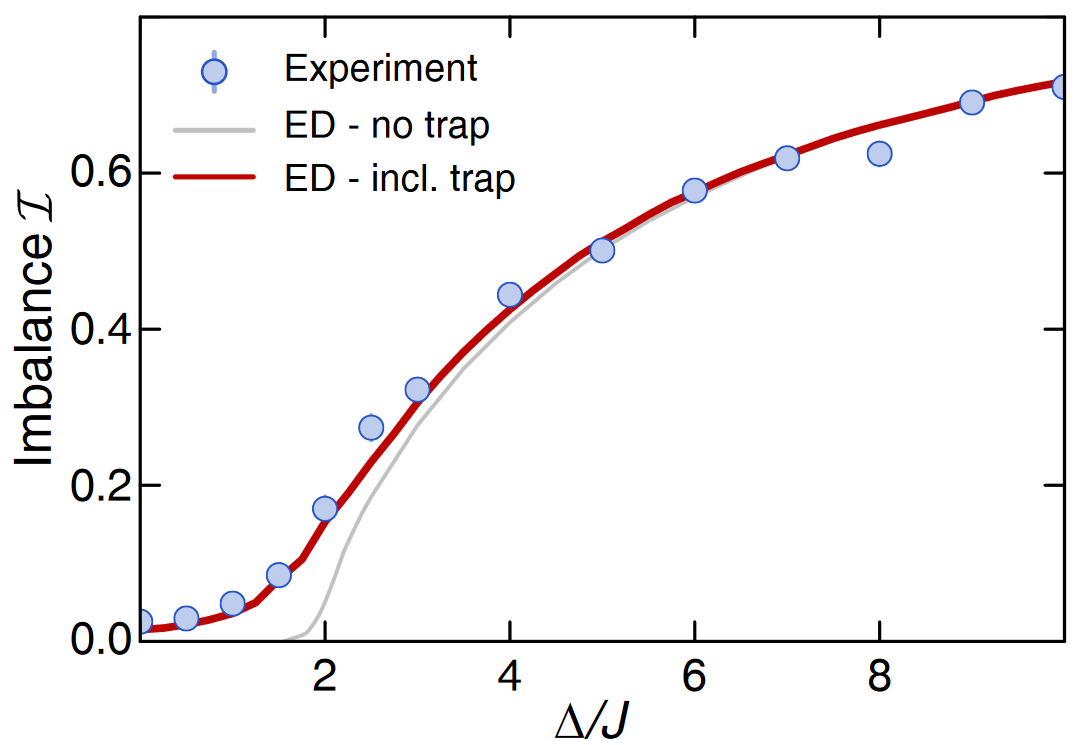
\includegraphics[align=c, width=0.35\textwidth]{imgs/MBL_exp_2.png}
    \caption{a) Time evolution of an initial charge-density wave. b) Stationary values of the imbalance $\mathcal{I}$ as a function of disorder $\Delta$ for non-interacting atoms \red{Основной вывод от этой картинки и этой статьи: есть локализация и термолизация. Взаимодействие влияет, но не столь принципиально.}}
    %\label{fig:}
\end{figure}


% \newpage
% Lorem ipsum dolor sit amet, consectetur adipisicing elit, sed do eiusmod
tempor incididunt ut labore et dolore magna aliqua. Ut enim ad minim veniam,
quis nostrud exercitation ullamco laboris nisi ut aliquip ex ea commodo
consequat. Duis aute irure dolor in reprehenderit in voluptate velit esse
cillum dolore eu fugiat nulla pariatur. Excepteur sint occaecat cupidatat non
proident, sunt in culpa qui officia deserunt mollit anim id est laborum.



Lorem ipsum dolor sit amet, consectetur adipisicing elit, sed do eiusmod
tempor incididunt ut labore et dolore magna aliqua. Ut enim ad minim veniam,
quis nostrud exercitation ullamco laboris nisi ut aliquip ex ea commodo
consequat. Duis aute irure dolor in reprehenderit in voluptate velit esse
cillum dolore eu fugiat nulla pariatur. Excepteur sint occaecat cupidatat non
proident, sunt in culpa qui officia deserunt mollit anim id est laborum.


% алхимик
% самурай
% провожающая
% убей или умри
% 
% 


